\documentclass{beamer}
\beamertemplatenavigationsymbolsempty
\usepackage{lmodern}
\usepackage{helvet}
  \renewcommand{\familydefault}{\sfdefault}
\usepackage{pdfcomment}
    \newcommand{\pdfnote}[1]{\marginnote{\pdfcomment[icon=note]{#1}}}

\mode<presentation>
{
  \usetheme{default}
}

\title{An Ageing Coder and His Ageing Code}
\author{Owen Campbell}
\date[DjangoCon Europe 2015]{3rd June, 2015\\DjangoCon Europe, Cardiff}

\AtBeginSection[]
{
  \begin{frame}<beamer>{Outline}
    \tableofcontents[currentsection]
  \end{frame}
}

\begin{document}

\begin{frame}
  \titlepage{}
\end{frame}

{
  \begin{frame}<beamer>{Outline}
    \tableofcontents
  \end{frame}
}

\section{The Ageing Coder}

  \begin{frame}{Primary School}
    \begin{columns}
      \column{0.67\textwidth}
        \begin{figure}
          \includegraphics[scale=0.25]{images/zx81}
        \end{figure}
      \column{0.33\textwidth}
        \begin{itemize}
          \item 1 KB Memory
          \item No permanent storage
        \end{itemize}
    \end{columns}
  \end{frame}

  \begin{frame}{Primary School}
    \begin{columns}
      \column{0.67\textwidth}
        \begin{figure}
          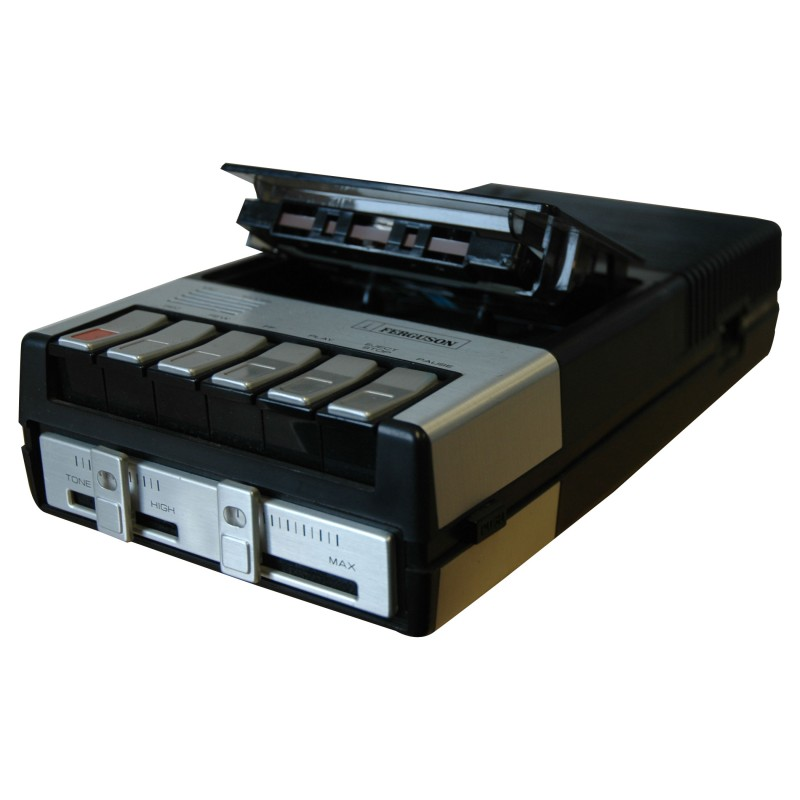
\includegraphics[scale=0.3]{images/3t07}
        \end{figure}
      \column{0.33\textwidth}
        \begin{figure}
          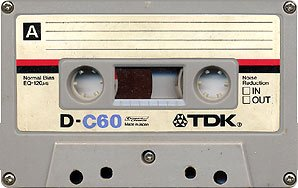
\includegraphics[scale=0.35]{images/tdkc60}
        \end{figure}
    \end{columns}
  \end{frame}

  \begin{frame}{Secondary School}
    \begin{columns}
      \column{0.67\textwidth}
        \begin{figure}
          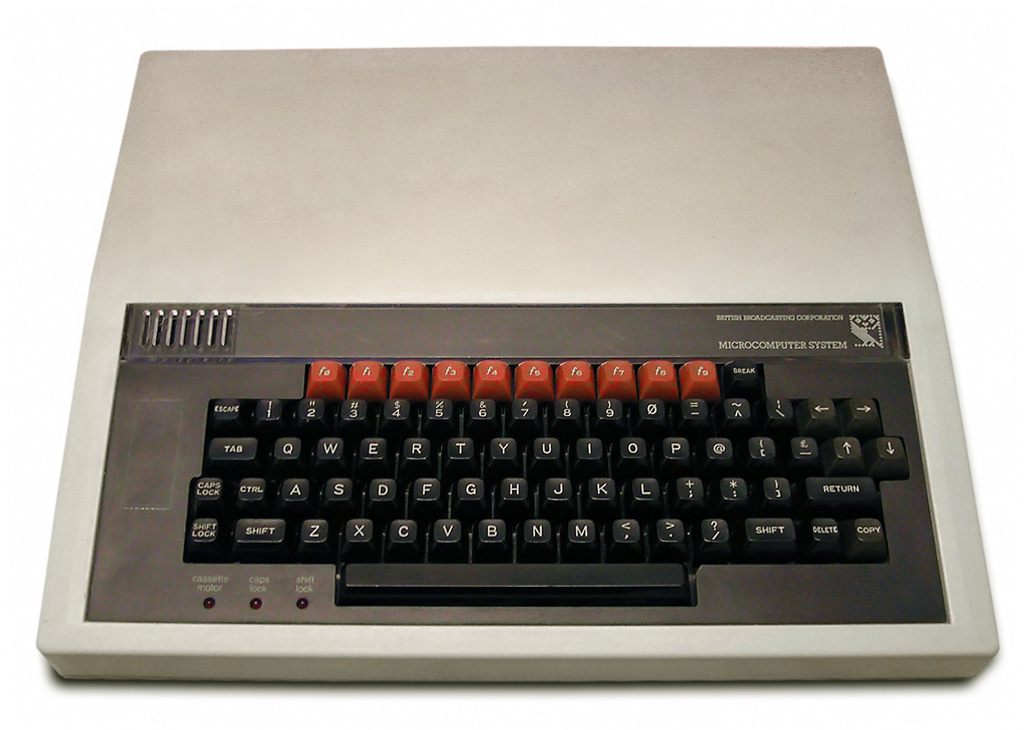
\includegraphics[scale=0.2]{images/bbc_micro}
        \end{figure}
      \column{0.33\textwidth}
      \begin{itemize}
          \item 32 KB Memory
          \item Still no permanent storage
        \end{itemize}
    \end{columns}
  \end{frame}

  \begin{frame}{University}
    \begin{figure}
      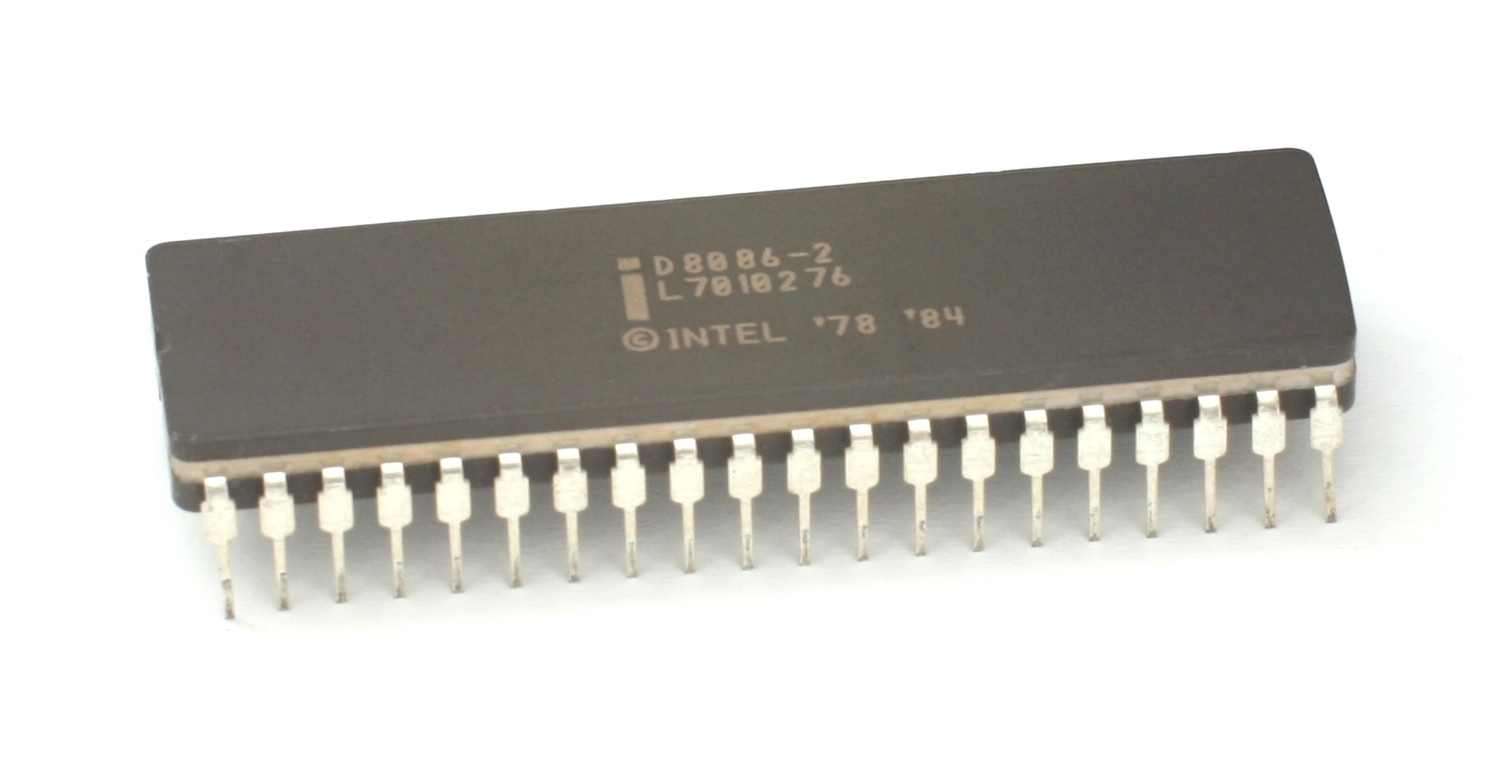
\includegraphics[scale=0.1]{images/8086}
      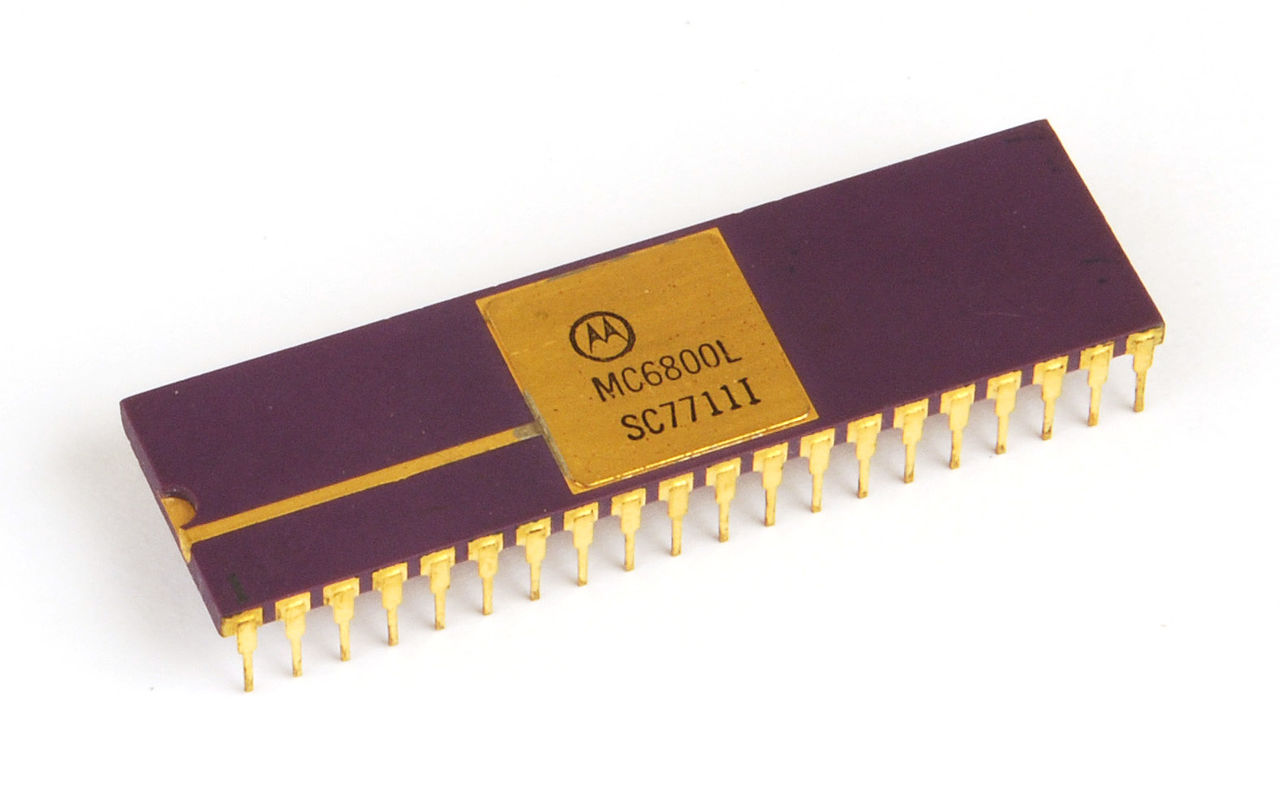
\includegraphics[scale=0.5]{images/6800}
    \end{figure}
    \pause
    \begin{figure}
      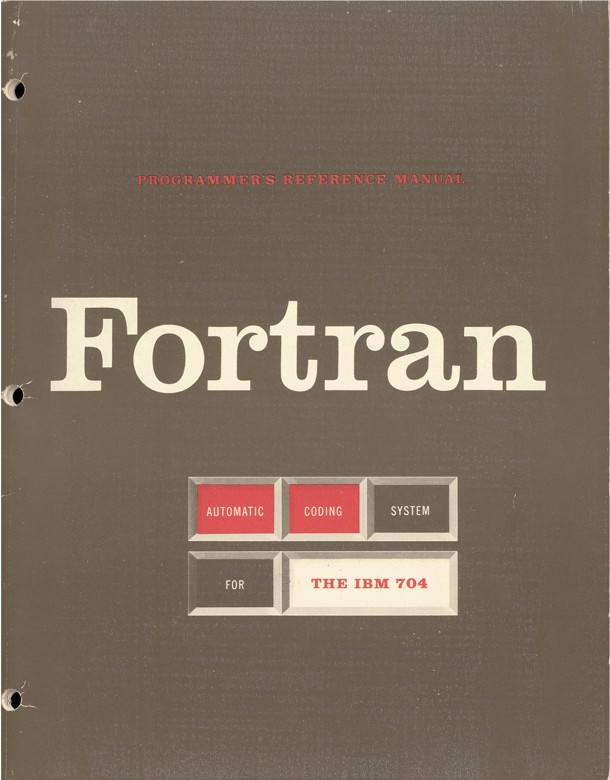
\includegraphics[scale=0.1]{images/fortran}
    \end{figure}
  \end{frame}

  \begin{frame}{And the Rest\ldots}
    \begin{columns}
        \column{0.5\textwidth}
          \begin{itemize}
            \item Lotus Approach
            \item Microsoft Access
            \item T-SQL
            \item PL/SQL
            \item PHP
            \item Perl
            \item Visual Basic
            \item Bash
          \end{itemize}
        \column{0.5\textwidth}
          \begin{itemize}
            \item Java
            \item ASP
            \item C
            \item C\#
            \item Ruby \& Rails
            \item Python \& Django
            \item Powershell
          \end{itemize}
      \end{columns}
  \end{frame}

\section{The Ageing Code}

  \begin{frame}{System}
    \begin{itemize}
      \item Accounting system for my Company
      \pause
      \item Database designed in mid 90s R\&D Project
      \pause
      \item Lotus Approach
      \pause
      \item Microsoft Access
      \pause
      \item Microsoft SQL Server + .NET client
      \item Logic coded as T-SQL Stored Procedures
    \end{itemize}
  \end{frame}

  \begin{frame}{Why Change?}
    \begin{itemize}
      \item Server Licence costs
      \pause
      \item Windows development environment
    \end{itemize}
  \end{frame}

\section{The Way Forward}

  \begin{frame}{Frameworks}
    \begin{itemize}
      \item Ruby \& Rails
      \pdfnote{
        Rails is opinionated - convention over configuration\textCR
        DB design doesn't fit with Rails convention}
      \item Scala \& Play
      \pdfnote{
        Scala was a joy to use\textCR
        Play is immature. Not enough standard packages
      }
      \item Javascript \& Node.js
      \item Python \& Django
      \pdfnote{
        Legacy database no problem\textCR
        Multiple database no problem\textCR
        Django Rest Framework\textCR
      }
    \end{itemize}
  \end{frame}

  \begin{frame}{Design}
    \begin{columns}
      \column{0.5\textwidth}
        \begin{itemize}
          \item Postgresql Database
          \item Django Rest Framework
          \item Logic as Django/DRF code
          \pause
        \end{itemize}
      \column{0.5\textwidth}
        \begin{itemize}
          \item AngularJS UI
          \item Coffeescript
          \item UI served separately
        \end{itemize}
    \end{columns}
  \end{frame}

  \section{Demo}

\end{document}
